% Field review prototype - what was built, how it works, how it did against truth
% Build:  latexmk -pdf fieldreview-prototype.tex   (or make fieldreview-prototype.pdf)
% Figures and tables: python ../python/validate_fieldreview.py  (make fieldreview-figures)
\documentclass[11pt,a4paper]{article}

\usepackage[margin=2.4cm]{geometry}
\usepackage{lmodern}
\usepackage[T1]{fontenc}
\usepackage[utf8]{inputenc}
\usepackage{microtype}
\usepackage{graphicx}
\usepackage{booktabs}
\usepackage{amsmath,amssymb}
\usepackage{xcolor}
\usepackage{caption}
\usepackage{subcaption}
\usepackage{enumitem}
\usepackage{tikz}
\usepackage{fancyhdr}
\usepackage{listings}
\usepackage{siunitx}

\definecolor{uavblue}{HTML}{1F4E79}
\definecolor{rulegrey}{HTML}{C8CCD2}
\definecolor{boxgrey}{HTML}{F4F5F7}

\usepackage[colorlinks=true,allcolors=uavblue]{hyperref}
\usetikzlibrary{arrows.meta,positioning}

\captionsetup{font=small,labelfont={bf,color=uavblue},width=0.92\textwidth}
\setlist{noitemsep,topsep=3pt}
\graphicspath{{figures/}}
\sisetup{detect-all}

\pagestyle{fancy}
\fancyhf{}
\renewcommand{\headrulewidth}{0.4pt}
\fancyhead[L]{\small\color{uavblue}UAV-RT \textbf{field review}}
\fancyhead[R]{\small\color{uavblue}Prototype report}
\fancyfoot[C]{\small\thepage}

\usepackage{titlesec}
\titleformat{\section}{\normalfont\Large\bfseries\color{uavblue}}{\thesection}{0.7em}{}
\titleformat{\subsection}{\normalfont\large\bfseries\color{uavblue}}{\thesubsection}{0.6em}{}

\lstset{basicstyle=\ttfamily\scriptsize, breaklines=true, breakindent=0pt,
        backgroundcolor=\color{boxgrey}, frame=single, rulecolor=\color{rulegrey},
        columns=fullflexible, keepspaces=true, xleftmargin=4pt, framexleftmargin=4pt}
\newcommand{\code}[1]{\texttt{\small #1}}
\newcommand{\dB}{\,\si{\decibel}}

\title{\vspace{-1.4cm}\color{uavblue}\textbf{UAV-RT field review}\\[2pt]
       \large\color{black}Prototype report: what was built, the methods, and how it did against known tag positions}
\author{\normalsize Dynamic and Active Systems Lab, Northern Arizona University}
\date{\normalsize 4 September 2026}

\begin{document}
\maketitle
\thispagestyle{fancy}
\vspace{-0.8cm}

\begin{center}
\fcolorbox{rulegrey}{boxgrey}{\begin{minipage}{0.94\textwidth}\small
\textbf{In one paragraph.} After a flight the operator wants to know where to walk next.
This prototype reads the pulse log TagTracker already writes, filters it by tag, time,
altitude and a map box, interpolates the signal strength over the flown area, and reports
the position where the received signal was strongest, in decimal degrees, together with any
other lobe worth knowing about, a bearing with a confidence, and contour lines. On the
flights where the true tag position is known, the strongest signal landed \SIrange{22}{41}{m}
from the tag on three well-sampled Cumbria flights and \SI{23}{m} and \SI{22}{m} on the final
flights of the two Ponui kiwi localisations, in every case on the downhill side of the tag, as
the field paper predicts. All numbers in
this document were produced by \code{python/validate\_fieldreview.py}; MATLAB was never run.
\end{minipage}}
\end{center}

\tableofcontents

\section{Why}

The field workflow that motivates this is in \code{docs/FIELD\_REVIEW.md} in the hub
repository. Between flights the operator lands, copies the pulse CSV off the Herelink to a
laptop, opens MATLAB, eyeballs the strongest signal, and reads coordinates off the screen
while cross-referencing a phone map. Each flight's result decides where the next one goes,
and the laptop round trip sits in the middle of that loop. The two New Zealand kiwi
localisations reported in Mohammadi, Shafer and Flikkema (2026) took four and three flights
each in exactly this loop.

The data is already on the Herelink. This prototype settles what the on-device analysis
should compute before anything is written into TagTracker. Its deliverable is settled
behaviour, not a user interface: the four questions the specification asks are answered in
Section~\ref{sec:answers}.

\section{What was built}

Everything lives in \code{uavrt\_postflight/python/} and is plain Python with numpy and
matplotlib, the same dependencies as the bench app.

\begin{center}\small
\begin{tabular}{@{}p{0.27\textwidth}p{0.68\textwidth}@{}}
\toprule
File & Purpose \\
\midrule
\code{analysis.py} & Shared primitives, new: \code{select\_pulses}, \code{grid\_spacing},
  \code{peak\_prominence}, \code{find\_peaks}, \code{edge\_distance}, \code{contour\_polylines} \\
\code{fieldreview.py} & \textbf{The entry point.} Pipeline, text report, figure, command line \\
\code{dem.py} & Terrain sampling for validation only; not part of the field feature \\
\code{validate\_fieldreview.py} & Runs every case with known truth and writes this document's figures and tables \\
\code{test\_fieldreview.py} & 51 checks on synthetic surfaces with known answers plus a real log \\
\code{kmzwrite.py} & Now takes its contour lines from the shared routine \\
\bottomrule
\end{tabular}
\end{center}

The bench app (\code{pulseplotter.py}) was not touched, and neither was TagTracker.
The log reader, the geodesy module, and the existing \code{build\_grid} and
\code{estimate\_bearing} are used exactly as they were.

\subsection{The control set}

Deliberately small, as the specification asks.

\begin{itemize}
\item \textbf{Tag.} Required in practice; the default is the most common tag in the log.
\item \textbf{Time window.} Opens on the flight proper: the takeoff climb and the landing
  descent are trimmed by the median-altitude rule the bench app already uses. The operator
  can widen or narrow it.
\item \textbf{Altitude window.} For the case the specification calls out, where the path
  recrosses the launch point and near-field pulses contaminate the surface.
\item \textbf{Spatial box.} The rectangle an operator would draw on the map. Implemented in
  the filter and on the command line; no drawing gesture in this prototype.
\item \textbf{Confirmed only.} On by default. Every log on disk contains only confirmed
  pulses, and the system reference says the CSV never receives unconfirmed ones, so this
  filter cannot be exercised on real data.
\end{itemize}

Grid spacing, smoothing window and the lobe thresholds are also on the command line, for the
configuration menu, not the main screen.

\subsection{What the operator gets}

Figure~\ref{fig:t42} is the figure for Cumbria tag 42 and the box below is the text report
for the same run. Positions are decimal degrees to five places, about \SI{1}{m}.

\begin{figure}[htbp]
\centering
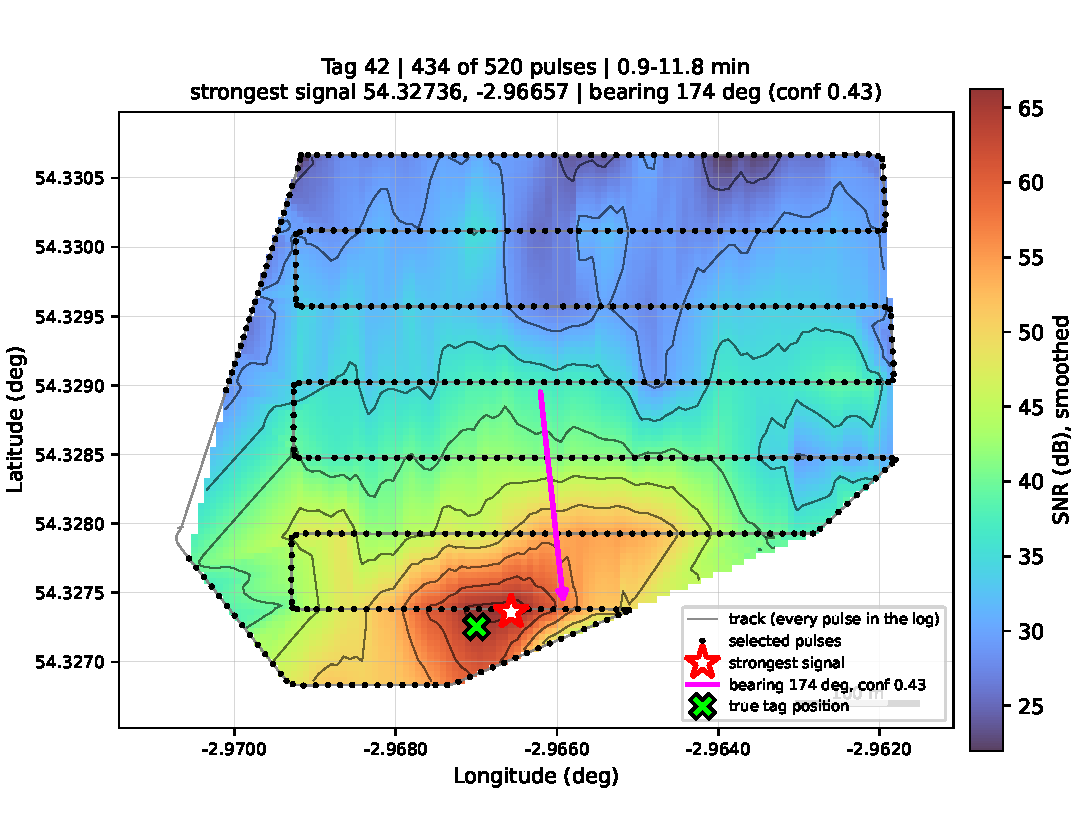
\includegraphics[width=0.95\textwidth]{fieldreview-cumbria-t42}
\caption{Cumbria, 21 November 2025, 11:08 log, tag 42. The raster is the interpolated
smoothed SNR, transparent outside the flown area; thin lines are contours; the grey line is
the track through every pulse in the log and the black dots the pulses that passed the
filters. The star is the strongest signal, the cross the true tag position, the arrow the
bearing from the centre of the selection. The strongest signal is \SI{30}{m} east-north-east
of the tag.}
\label{fig:t42}
\end{figure}

\lstinputlisting{figures/fieldreview-report-t42.txt}

Three things the report always does. It labels the position \emph{strongest signal} and
says on every run that this is not the tag position and why. It flags a \emph{weak} surface,
one whose peak is less than \SI{10}{dB} above the median of the surface, as unreliable. And it
says when the peak sits on the edge of the flown area, because then the surface was still
rising when the survey ran out and the useful advice is to fly further that way.

\section{Methods}

\subsection{Local frame and interpolation}

Positions are converted to a local east--north frame anchored on the first pulse of the log,
using the WGS84 meridional and normal radii of curvature at the reference latitude:
\begin{equation}
x_E = R_N \cos\phi_0\,(\lambda-\lambda_0), \qquad y_N = R_M\,(\phi-\phi_0),
\end{equation}
which agrees with a rigorous ECEF transform to under \SI{5}{cm} over a kilometre. The
smoothed SNR is interpolated onto a regular grid by linear interpolation over the Delaunay
triangulation of the pulse positions (\code{build\_grid}, unchanged), and is undefined outside
their convex hull.

One property of that surface matters for everything that follows: \textbf{the maximum of a
piecewise-linear interpolant is always at a vertex.} The strongest-signal position is
therefore always the position of a pulse, after smoothing, and never a point between flight
lines. Its cross-track resolution is the transect spacing. This is also why the grid spacing
barely moves the reported position (Section~\ref{sec:sensitivity}): the grid only quantises
where that vertex is sampled.

\subsection{Smoothing}

SNR is smoothed in flight order with the bench app's centred moving mean over $k=6$ pulses,
\begin{equation}
\bar v_i = \frac{1}{|W_i|}\sum_{j\in W_i} v_j, \qquad
W_i = \{\,j : i-\lfloor k/2\rfloor \le j \le i + k - \lfloor k/2\rfloor - 1\,\},
\end{equation}
windows shrinking at the ends and NaNs omitted, matching MATLAB's \code{movmean}. This is
smoothing along the track, not across it.

\subsection{Grid spacing from the data}
\label{sec:spacing}

A fixed spacing in metres looks wrong on one of a \SI{60}{m} lawnmower and a kilometre
survey. Two things bound a sensible spacing. The surface carries no detail finer than the
pulse spacing, so half the median distance $d$ between consecutive pulses is the natural
starting point; it is also the PI's rule of thumb (about \SI{10}{m} at \SI{15}{mph} and
\SI{1.5}{s} per pulse). And the map is drawn at a fixed size whatever was flown, so fewer than
about 60 cells across the longer side $L$ looks blocky and more than about 300 is invisible
and slow:
\begin{equation}
\Delta = \operatorname{clip}\!\left(\tfrac{d}{2},\; \tfrac{L}{300},\; \tfrac{L}{60}\right),
\qquad \Delta \ge \SI{1}{m}.
\label{eq:spacing}
\end{equation}
Consecutive pulses at exactly the same position, which the 2023 logs produce because the
position feed was slower than the pulse rate, are left out of the median. The existing cell
cap in \code{build\_grid} still applies on top. Table~\ref{tab:spacing} shows what the rule
chose on every dataset on disk.

\begin{table}[htbp]
\centering
\resizebox{\textwidth}{!}{\begin{tabular}{lrrrrlrr}
\toprule
Dataset & Pulses & Extent (m) & Step (m) & Grid (m) & Bound & Cells & Time (s) \\
\midrule
Cumbria 09:35 (largest survey) & 265 & 1060 $\times$ 1140 & 14.9 & 7.4 & step/2 & 22022 & 0.02 \\
Cumbria 11:08 & 434 & 570 $\times$ 428 & 10.0 & 5.0 & step/2 & 9804 & 0.03 \\
Ponui case 2 flight 3 & 328 & 223 $\times$ 316 & 4.9 & 2.5 & step/2 & 11739 & 0.03 \\
Ponui case 1 flight 4 & 363 & 184 $\times$ 159 & 4.7 & 2.4 & step/2 & 5451 & 0.01 \\
Raymond Park scan 2025-01-13 & 524 & 262 $\times$ 296 & 5.0 & 2.5 & step/2 & 12614 & 0.04 \\
Engineering lawn lawnmower 2025-01-03 & 166 & 67 $\times$ 65 & 3.7 & 1.1 & extent/60 & 3599 & 0.01 \\
Raymond Park monopole 2024-10-11 & 655 & 91 $\times$ 469 & 2.3 & 1.6 & extent/300 & 17759 & 0.04 \\
NAVHDA 2023-08-18 (1 km, headerless) & 1012 & 1003 $\times$ 1087 & 11.1 & 5.5 & step/2 & 35854 & 0.04 \\
\bottomrule
\end{tabular}
}
\caption{Grid spacing chosen by equation~\eqref{eq:spacing} across the datasets on disk, the
bound that decided it, and the time for the whole review on the development laptop. Every
survey landed on half the pulse spacing; only the two smallest flights and the 2023 log with
duplicated positions fell back to an extent bound.}
\label{tab:spacing}
\end{table}

\subsection{Strongest signal, and other lobes}
\label{sec:lobes}

The strongest signal is the highest cell of the surface. The question the specification asks
is what to do when the surface has two lobes: two transmitters on one channel, a reflection,
or a transit leg. Reporting only the highest cell hides the other; reporting every local
maximum drowns the operator, because a real surface has hundreds of them (163 on the surface
of Figure~\ref{fig:lobes}).

What separates a second lobe from a wrinkle on the first is its \textbf{topographic
prominence}: how far the surface has to drop from that maximum before it can climb to
something taller. For a local maximum $p$ and any higher point $q$,
\begin{equation}
\operatorname{prom}(p) = z(p) - \max_{\gamma:\,p\to q,\; z(q)>z(p)}\;\min_{c\in\gamma} z(c),
\end{equation}
the height of $p$ above the highest saddle that connects it to higher ground. The global
maximum has no higher ground; its prominence is taken as its height above the lowest cell.

\begin{center}
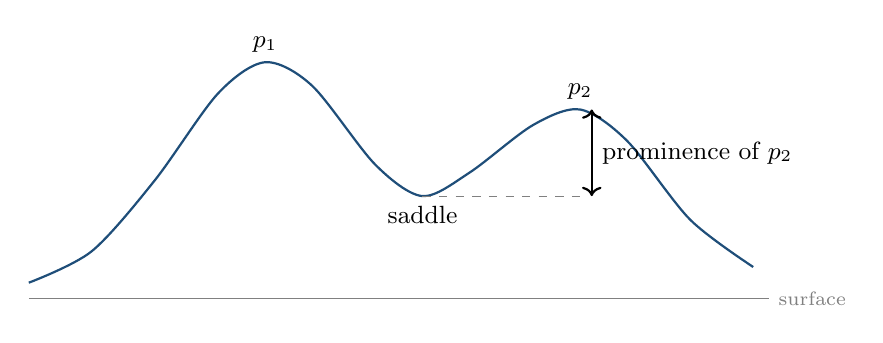
\begin{tikzpicture}[x=1cm,y=1cm,scale=1.0]
\draw[thick,color=uavblue] plot[smooth] coordinates
  {(0,0.2) (0.8,0.6) (1.6,1.5) (2.4,2.6) (3.0,3.0) (3.6,2.7) (4.4,1.7) (5.0,1.3) (5.6,1.6) (6.4,2.2) (7.0,2.4) (7.6,2.0) (8.4,1.0) (9.2,0.4)};
\draw[dashed,gray] (5.0,1.3) -- (7.0,1.3);
\draw[<->,thick] (7.15,1.3) -- (7.15,2.4) node[midway,right,font=\small] {prominence of $p_2$};
\node[above,font=\small] at (3.0,3.0) {$p_1$};
\node[above,font=\small] at (7.0,2.4) {$p_2$};
\node[below,font=\small] at (5.0,1.3) {saddle};
\draw[gray,thin] (0,0) -- (9.4,0);
\node[right,font=\scriptsize,gray] at (9.4,0) {surface};
\end{tikzpicture}
\end{center}

It is computed as zero-dimensional persistence. Cells are visited from the highest down. A
cell with no visited 8-neighbour starts a new component and is a local maximum; otherwise it
joins the components of its visited neighbours, and when that joins two components the one
with the lower peak dies at the current level, its prominence being its peak minus that
level. Union-find with path compression makes this $O(N\log N)$ for the sort and near-linear
after it; NaN cells are never visited, so nothing crosses the edge of the flown area. On the
grids here it takes a few tens of milliseconds.

A local maximum is then \textbf{reported as a lobe} when
\begin{equation}
z_{\max} - z(p) \le W = \SI{10}{dB}
\quad\text{and}\quad
\operatorname{prom}(p) \ge P = \SI{2}{dB},
\end{equation}
at most three in all, ranked by height. Each carries how far below the strongest it is, the
distance and compass direction from the strongest, and its prominence. An optional minimum
separation in metres is implemented but off. The thresholds were chosen from the sweep in
Table~\ref{tab:lobes}: at the \SI{3}{dB} window first proposed, no well-sampled flight ever
reports a second lobe, including the two-transmitter surface where the second transmitter is
\SI{6.5}{dB} down; at \SI{10}{dB} and \SI{2}{dB} that surface reports both sites, every clean
bullseye still reports one lobe, and the flights that spray lobes are the ones already
flagged weak.

Two further flags come from the same surface. \textbf{Weak:} the peak is less than
\SI{10}{dB} above the median of the surface, so the surface is essentially flat and its
maximum is noise; every flight in the validation where the tag was only heard near the noise
floor was caught by this. \textbf{Edge:} the peak is within two cells of a NaN cell or the
array border, i.e.\ of the hull of the flown area.

\subsection{Bearing}

Unchanged from the bench app and restated here because it is on the screen. With $\mathbf{g}
= \nabla z$ the gradient of the surface, which points uphill toward the tag, and cells
outside the hull excluded,
\begin{equation}
\mathbf{R} = \frac{\sum_i |\mathbf{g}_i|\,\hat{\mathbf{g}}_i}{\sum_i |\mathbf{g}_i|}
           = \frac{\sum_i \mathbf{g}_i}{\sum_i |\mathbf{g}_i|},
\qquad
\theta = \operatorname{atan2}(R_x, R_y),
\qquad
c = |\mathbf{R}|,
\qquad
\sigma = \sqrt{-2\ln c}.
\end{equation}
$\theta$ is a compass bearing, $c$ the confidence in $[0,1]$ (1 when every cell agrees) and
$\sigma$ the circular standard deviation. The magnitude weight cancels the normalisation, so
the direction is that of the mean gradient; what the circular form adds is $c$. The bearing is
anchored at the centre of the selected pulses.

The validation adds one thing worth knowing about it. When the tag is \emph{inside} the flown
area the surface is a bullseye, the gradients point every way, and the confidence collapses:
0.13 on the final Ponui flight, with the bearing \SI{115}{\degree} wrong on the flight before.
The bearing is the right tool when the tag is beyond the survey and the surface is a slope;
the peak is the right tool when it is inside. The confidence tells the two apart.

\subsection{Contours}

Levels are the same nice values matplotlib would pick for an integer level count, kept
strictly inside the data range. The lines are extracted with \code{contourpy}, the library
matplotlib itself uses, as plain coordinate arrays, first in local metres and then in
lat/lon, with no figure involved, so a map renderer, the KML writer and the plot all draw
the same lines. The KMZ writer now uses this routine.

\subsection{Terrain check, validation only}

The field paper's explanation for the offset is propagation geometry: the monopole's
toroidal pattern and the terrain put the strongest received signal slightly downhill of the
tag. To test that, \code{dem.py} samples two elevation models that need no login: the
Environment Agency's \SI{1}{m} LiDAR terrain model for Cumbria, fetched by lat/lon box from
their WCS service, and Copernicus GLO-30 (\SI{30}{m}) for Ponui, a surface model that
includes tree canopy. At the true tag position a plane $z \approx a + b\,e + c\,n$ is fitted
to the cells within \SI{25}{m} (EA) or \SI{60}{m} (Copernicus); the downhill direction is
$\operatorname{atan2}(-b,-c)$. The report gives $\Delta z = z(\text{peak}) - z(\text{tag})$
and the component of the tag-to-peak offset along the downhill direction. $\Delta z$ is the
more direct of the two: the terrain is not a plane over \SI{30}{m}, and on the Cumbria knoll
the two disagree in sign.

\section{Results}

\subsection{Ground truth}

\begin{center}\small
\begin{tabular}{@{}p{0.24\textwidth}p{0.23\textwidth}p{0.27\textwidth}p{0.18\textwidth}@{}}
\toprule
Site & Position (lat, lon) & Source & Note \\
\midrule
Cumbria tags 40, 41 & 54.326601, $-$2.9684094 & the PI's \path{Tag42_Above_60m_PROCESS.m}, beside the logs & one site, two tags \\
Cumbria tags 42, 43 & 54.327254, $-$2.966997 & same & one site, two tags \\
Ponui case 1 kiwi & $-$36.887851, 175.184943 & PI's field notebook, 4 Sep 2026 & under a bush; may have moved during the day \\
Ponui case 2 kiwi & $-$36.886383, 175.178570 & PI's field notebook, 4 Sep 2026 & in a burrow \\
\bottomrule
\end{tabular}
\end{center}

The paper's case 1 is four ten-minute flights on one day; case 2 is three. The Ponui logs
match that on 20 March (tag 12, four flights of 8--14 minutes, the first with its strongest
detections \SI{1.5}{min} after takeoff, as the paper describes) and 23 March (tag 24, three
flights with median altitudes stepping 36, 25, \SI{3}{m}). The case 1 position was first
supplied with a digit wrong; the flights themselves pointed at a position \SI{29}{m} from the
one the notebook then gave, which is a small validation of its own.

\subsection{Against truth}

\begin{table}[htbp]
\centering
\resizebox{\textwidth}{!}{\begin{tabular}{lrrrrrrrrr}
\toprule
Case & Pulses & Peak SNR & Contrast & Offset & Dir. & $\Delta z$ & Downhill & Bearing err. & Lobes \\
\midrule
Cumbria 11:08, tag 42 & 434 & 66 dB & 31 dB & 30 m & ENE & -6 m & -4 m & -21$^\circ$ & 1 \\
Cumbria 11:08, tag 43 (weak) & 13 & 11 dB & 5 dB & 481 m & NE & -32 m & -285 m & +166$^\circ$ & 1 \\
Cumbria 11:08, tag 40 & 429 & 49 dB & 25 dB & 85 m & N & +2 m & -29 m & -37$^\circ$ & 2 \\
Cumbria 11:08, tag 41 (weak) & 61 & 11 dB & 9 dB & 562 m & NE & -33 m & +160 m & +130$^\circ$ & 3 \\
Cumbria 09:35, tag 42 (edge) & 265 & 56 dB & 14 dB & 124 m & ESE & -23 m & +64 m & +71$^\circ$ & 2 \\
Cumbria 09:35, tag 40 (weak) & 268 & 35 dB & 8 dB & 190 m & E & -15 m & +174 m & +30$^\circ$ & 3 \\
Cumbria 13:05, tag 42 & 451 & 63 dB & 27 dB & 22 m & NE & -3 m & -7 m & -15$^\circ$ & 1 \\
Cumbria 13:05, tag 40 & 449 & 48 dB & 23 dB & 85 m & N & +3 m & -34 m & -17$^\circ$ & 2 \\
Cumbria 14:12, tag 42 & 451 & 61 dB & 21 dB & 41 m & ENE & -7 m & -7 m & -12$^\circ$ & 1 \\
Cumbria 14:12, tag 40 & 452 & 48 dB & 19 dB & 127 m & NE & +2 m & +60 m & -17$^\circ$ & 1 \\
Ponui case 1, flight 1 (edge) & 179 & 34 dB & 21 dB & 195 m & NE & +18 m & +184 m & +40$^\circ$ & 2 \\
Ponui case 1, flight 2 (weak) & 314 & 38 dB & 9 dB & 158 m & NNE & +18 m & +156 m & +0$^\circ$ & 3 \\
Ponui case 1, flight 3 & 346 & 45 dB & 16 dB & 42 m & NNE & -19 m & +42 m & +86$^\circ$ & 2 \\
Ponui case 1, flight 4 & 363 & 51 dB & 15 dB & 23 m & NNE & -11 m & +23 m & +64$^\circ$ & 2 \\
Ponui case 2, flight 1 (weak) & 86 & 20 dB & 7 dB & 119 m & ESE & +1 m & +64 m & -28$^\circ$ & 2 \\
Ponui case 2, flight 2 & 293 & 32 dB & 17 dB & 36 m & SE & -3 m & +29 m & -115$^\circ$ & 1 \\
Ponui case 2, flight 3 & 328 & 32 dB & 18 dB & 22 m & E & -2 m & +4 m & +25$^\circ$ & 1 \\
\bottomrule
\end{tabular}
}
\caption{Every case with a known tag position, at the defaults. Offset is from the tag to
the strongest signal, with its compass direction; $\Delta z$ is the elevation of the peak
minus that of the tag; downhill is the component of the offset along the local downhill
direction at the tag, positive when the peak is on the downhill side; bearing error is the
estimate minus the true bearing from the centre of the selection to the tag. \emph{Weak}
and \emph{edge} are the report's own flags.}
\label{tab:cases}
\end{table}

\paragraph{Cumbria tag 42, the well-sampled case.} On the three \SI{60}{m}--\SI{120}{m}
surveys of the same box the strongest signal is \SI{30}{m}, \SI{22}{m} and \SI{41}{m} from
the tag, all to the north-east, all \SIrange{3}{7}{m} lower in elevation. The tag sits on a
small knoll (Figure~\ref{fig:terrain}); the peak is on its slope. The 09:35 flight, flown
higher and over four times the area, gives \SI{124}{m} with the edge flag set: a coarse
first pass, which is what it was.

\paragraph{Cumbria tag 40, the tag beyond the survey.} The tag is \SI{85}{m} south of the
southernmost transect, and the peak lands on that transect directly north of it on all
three flights (Figure~\ref{fig:t40}). This is the cross-track limit of the method:
the surface cannot peak where nothing flew. The one leg that did pass within \SI{25}{m} of the
tag, the outbound leg at low altitude, heard it \emph{more weakly} than the transect
\SI{85}{m} away; that is the overhead null of the vertical monopole, and it is the same
physics as the downhill offset. Without smoothing the single strongest pulse is on that
near leg, \SI{33}{m} from the tag.

\paragraph{Cumbria tags 41 and 43, the weak case.} Both were only heard near the noise
floor, \SI{11}{dB} peak and \SIrange{5}{9}{dB} contrast. The positions are \SIrange{480}{560}{m}
wrong and the report says so: weak, at the edge, with the bearing \SI{130}{\degree} off.
Figure~\ref{fig:t41} is what an operator would see.

\paragraph{Ponui case 2.} The three flights converge 119, 36, \SI{22}{m}
(Figure~\ref{fig:ponui2}); the first is flagged weak and at the edge, the last two are
clean bullseyes. The final peak is \SI{22}{m} east of the burrow and \SI{2.5}{m} lower. The
paper reports ``within about \SI{20}{m}, uphill as expected''.

\paragraph{Ponui case 1.} The four flights converge 195, 158, 42, \SI{23}{m}
(Figure~\ref{fig:ponui1}); the last peak is \SI{23}{m} north-north-east of the bush and
\SI{11}{m} lower, on a steep hillside. The paper reports ``about \SI{30}{m}''. The first two
flights, where the bird may still have been elsewhere, put the peak \SI{18}{m} \emph{above}
the final position; the two that found it put it below.

\begin{figure}[htbp]
\centering
\begin{subfigure}[t]{0.49\textwidth}
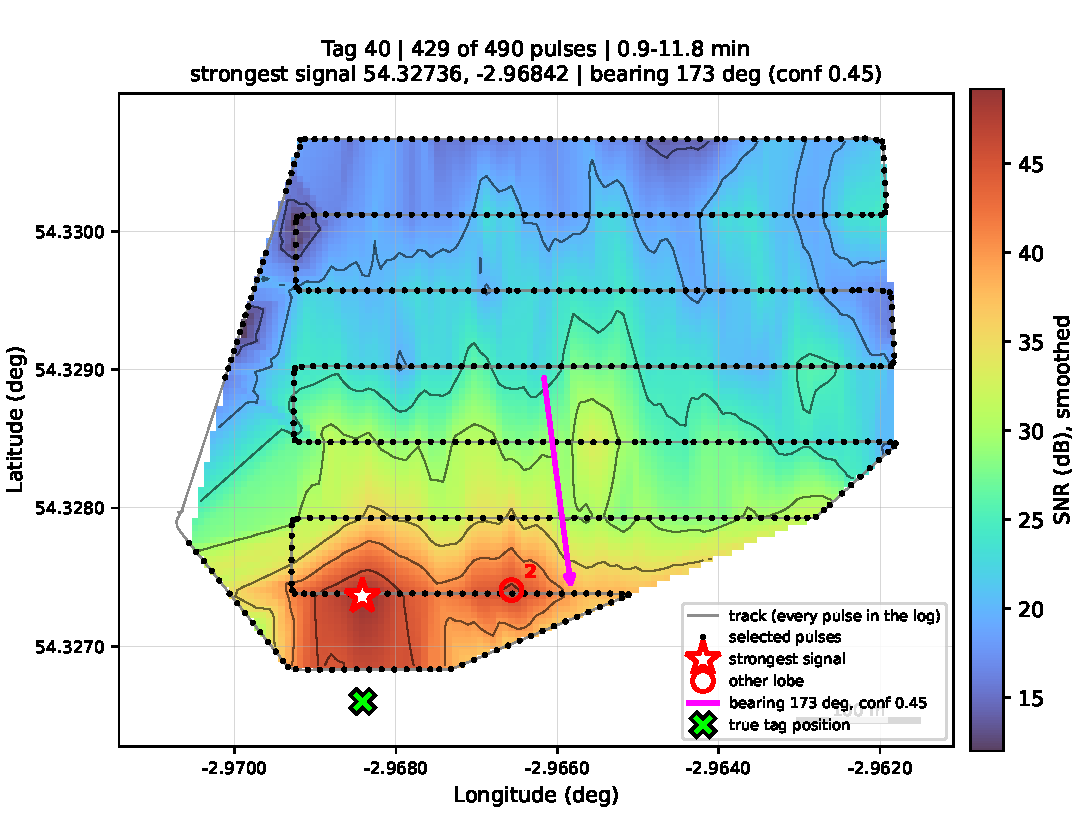
\includegraphics[width=\textwidth]{fieldreview-cumbria-t40}
\caption{Tag 40: the tag lies beyond the last transect, so the peak sits on it.}
\label{fig:t40}
\end{subfigure}\hfill
\begin{subfigure}[t]{0.49\textwidth}
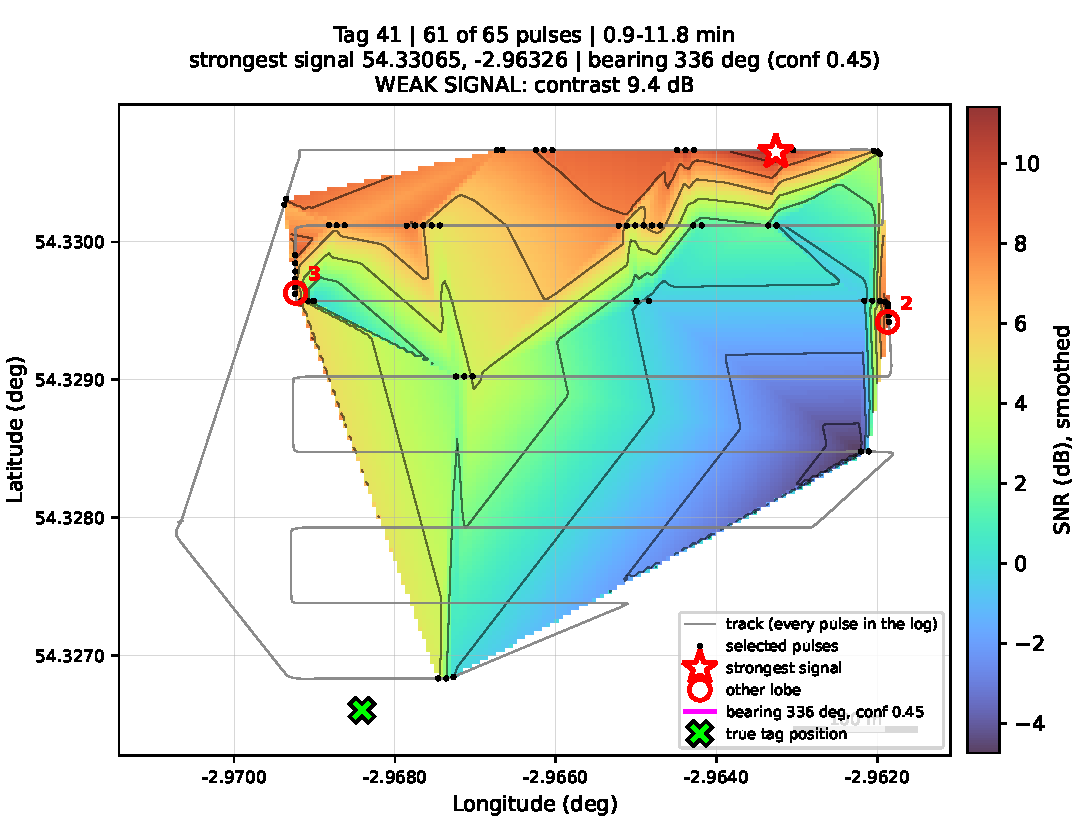
\includegraphics[width=\textwidth]{fieldreview-cumbria-t41}
\caption{Tag 41: heard only near the noise floor; flagged weak.}
\label{fig:t41}
\end{subfigure}
\caption{Two behaviours the report flags, same flight as Figure~\ref{fig:t42}.}
\end{figure}

\begin{figure}[htbp]
\centering
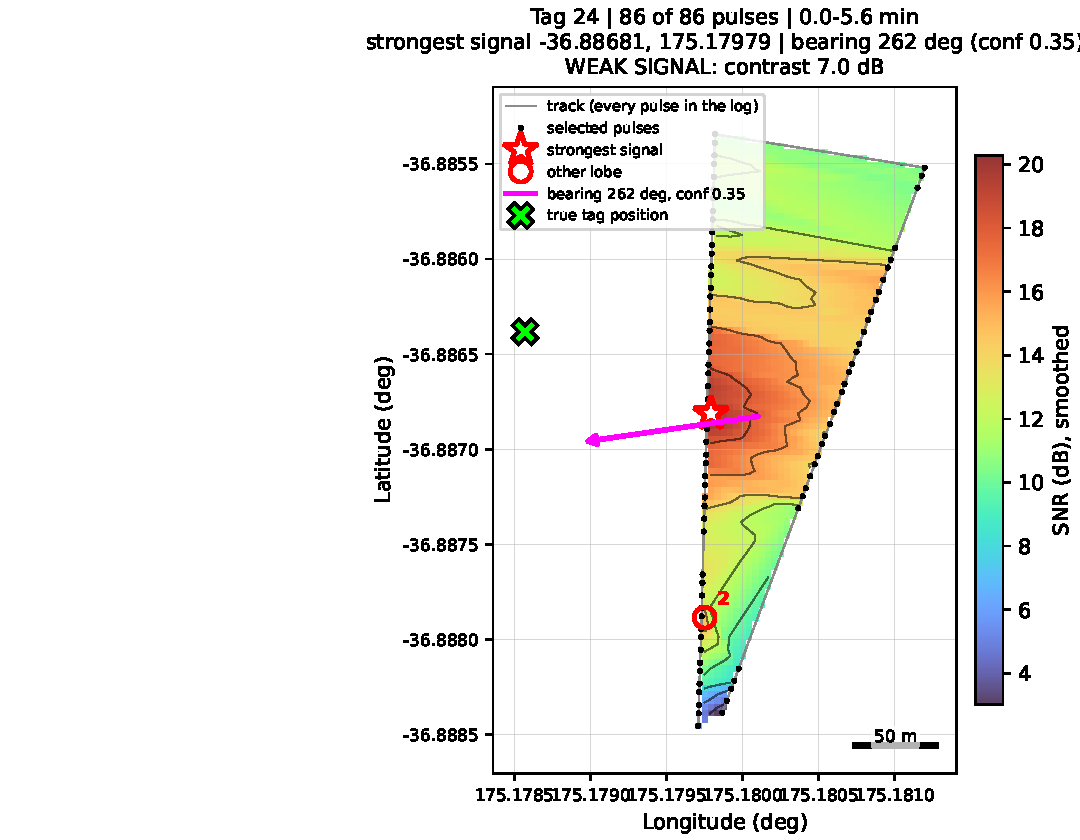
\includegraphics[width=0.325\textwidth]{fieldreview-ponui-c2-f1}\hfill
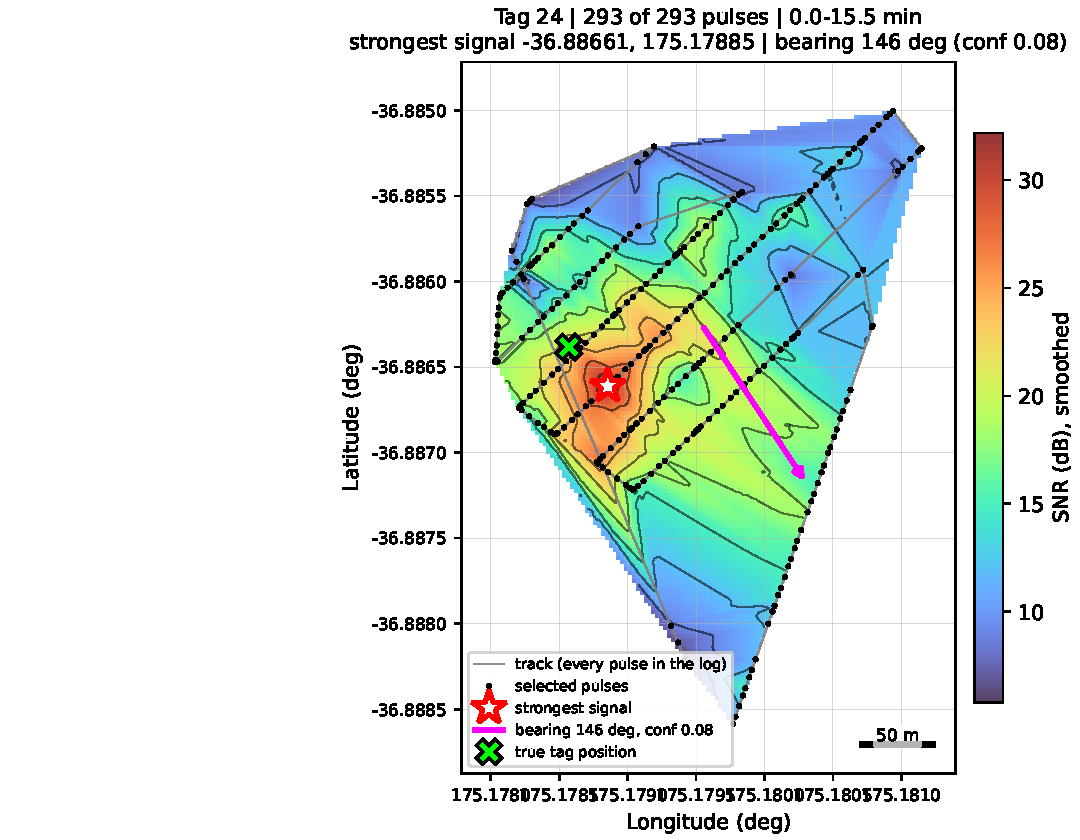
\includegraphics[width=0.325\textwidth]{fieldreview-ponui-c2-f2}\hfill
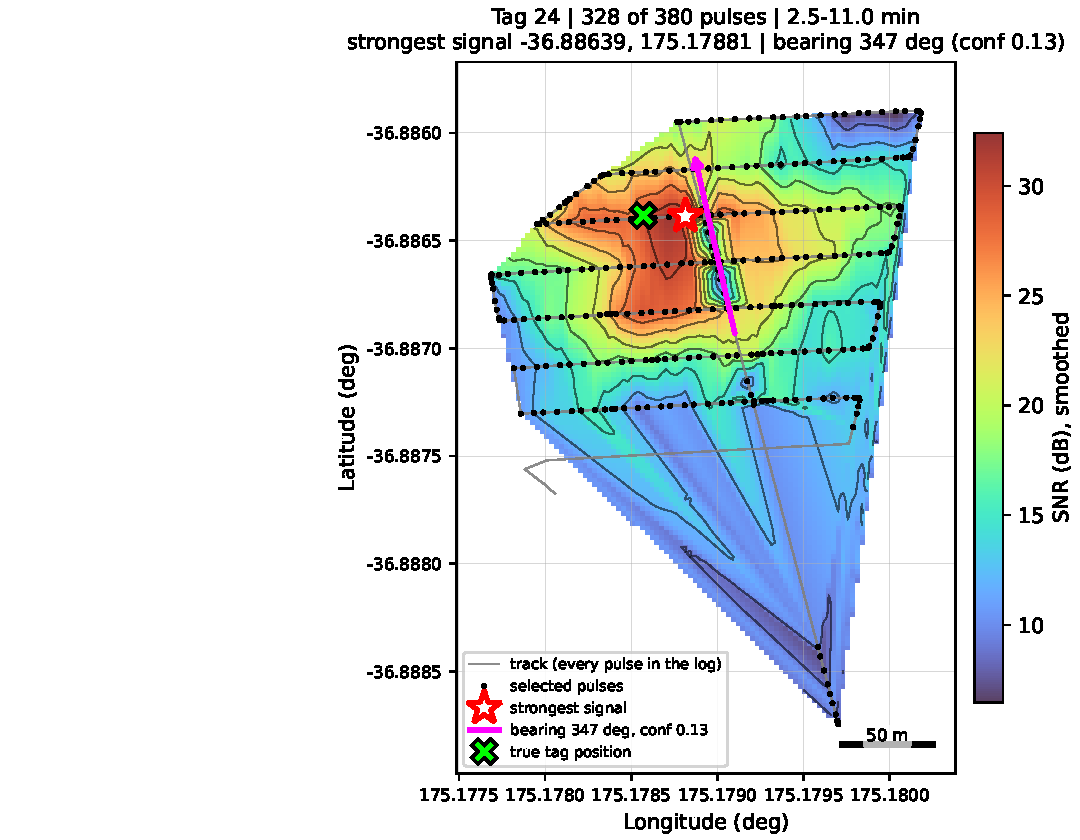
\includegraphics[width=0.325\textwidth]{fieldreview-ponui-c2-f3}
\caption{Ponui case 2, the three flights of 23 March 2025 on tag 24, converging 119, 36,
\SI{22}{m} on the burrow. The long wedge in the third panel is the convex hull stretched over
the never-flown area between the grid and the transit leg; the spatial box is the control
that cuts it.}
\label{fig:ponui2}
\end{figure}

\begin{figure}[htbp]
\centering
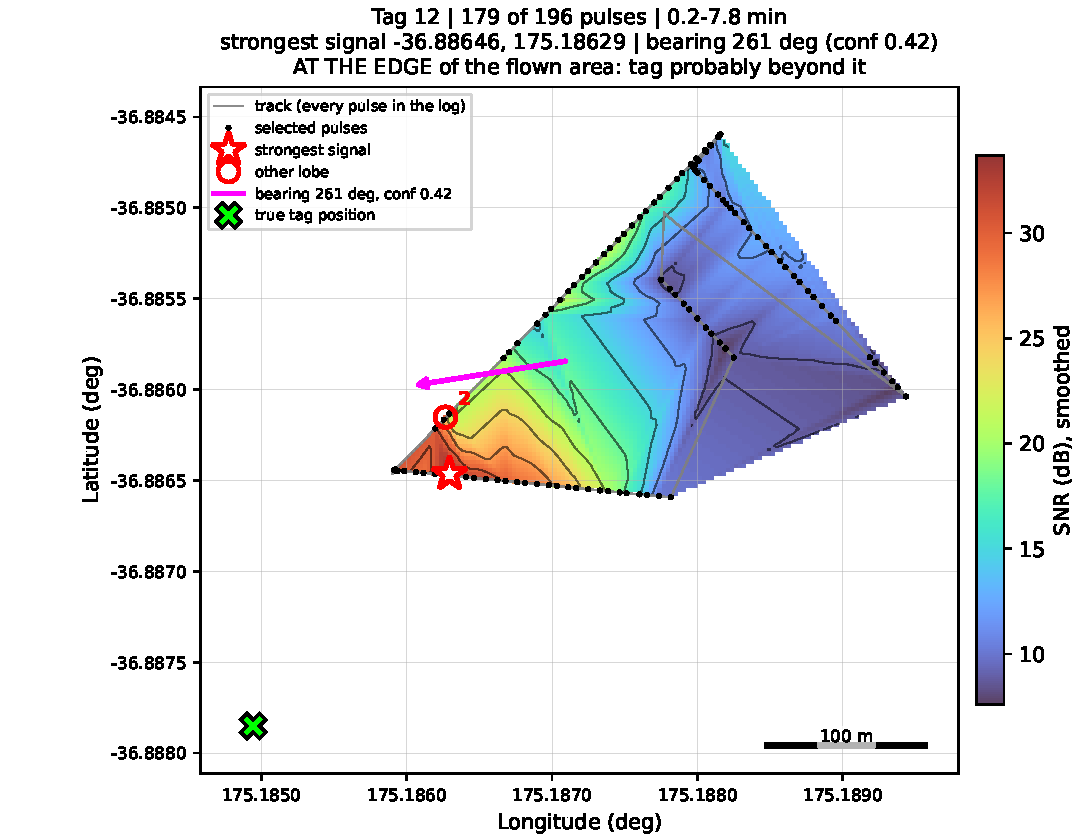
\includegraphics[width=0.49\textwidth]{fieldreview-ponui-c1-f1}\hfill
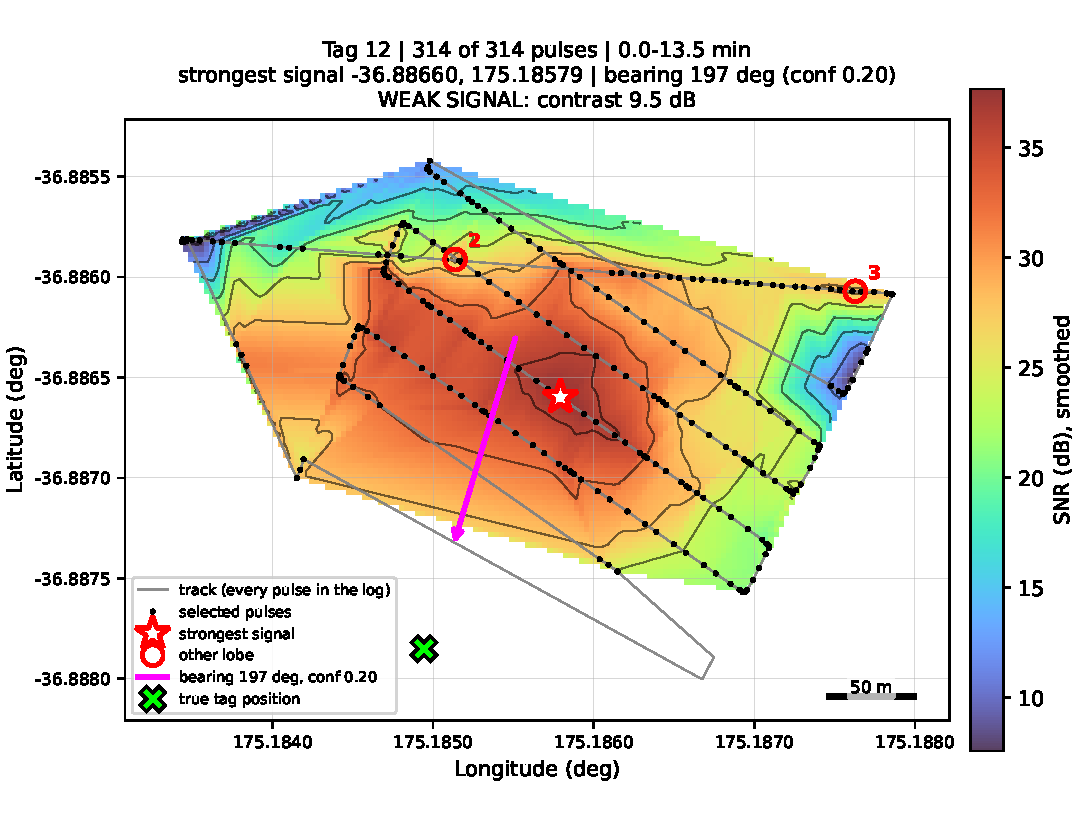
\includegraphics[width=0.49\textwidth]{fieldreview-ponui-c1-f2}\\[2pt]
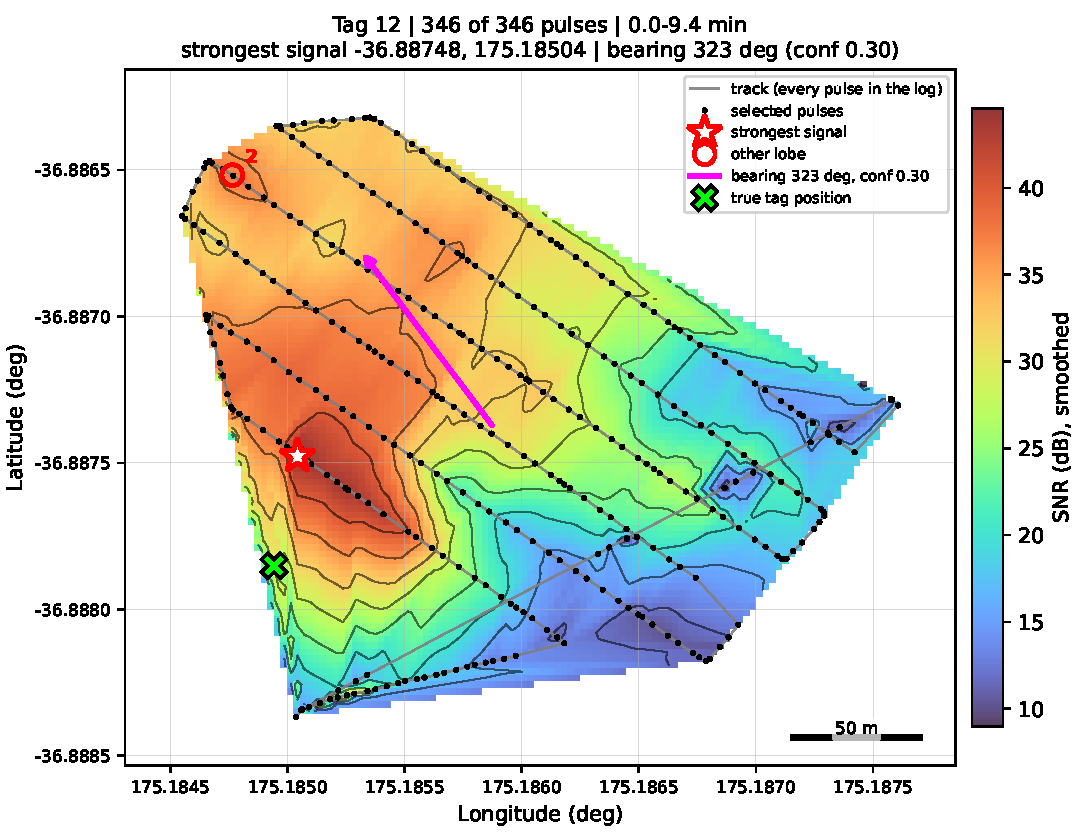
\includegraphics[width=0.49\textwidth]{fieldreview-ponui-c1-f3}\hfill
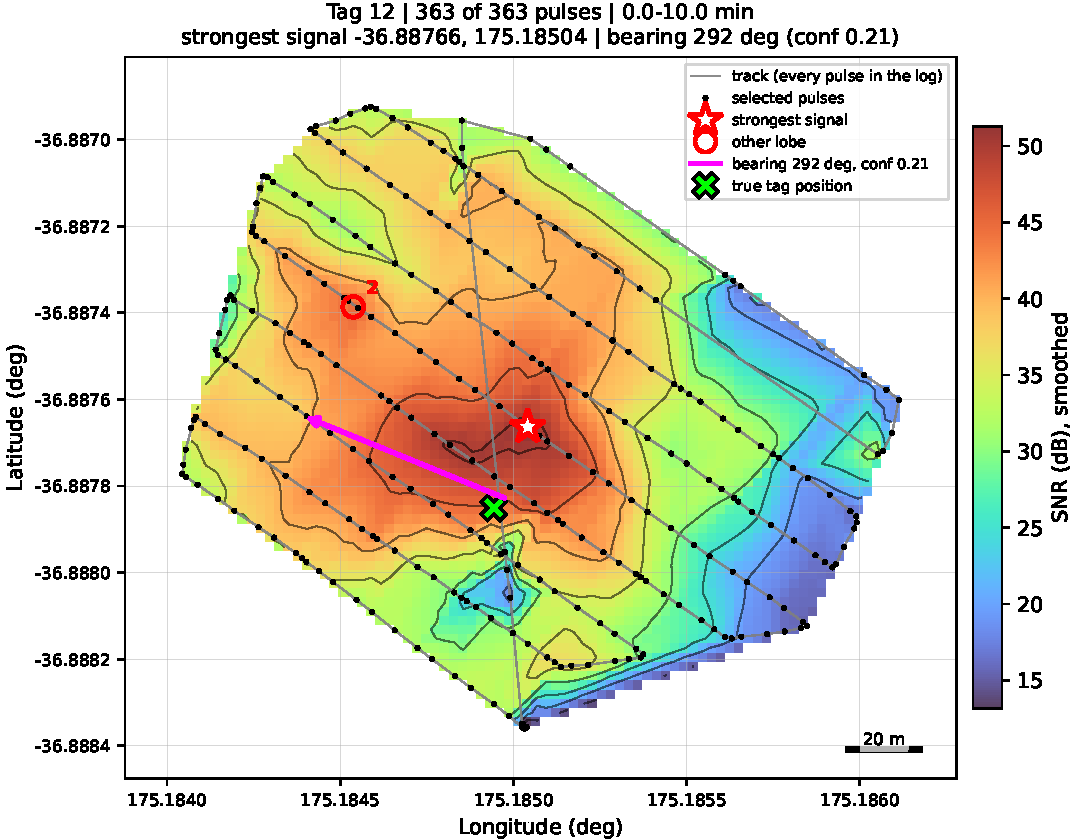
\includegraphics[width=0.49\textwidth]{fieldreview-ponui-c1-f4}
\caption{Ponui case 1, the four flights of 20 March 2025 on tag 12, converging 195, 158,
42, \SI{23}{m} on the bush. The first flight's strongest signal is at the edge of its survey,
as the paper describes.}
\label{fig:ponui1}
\end{figure}

\subsection{Downhill?}

\begin{figure}[htbp]
\centering
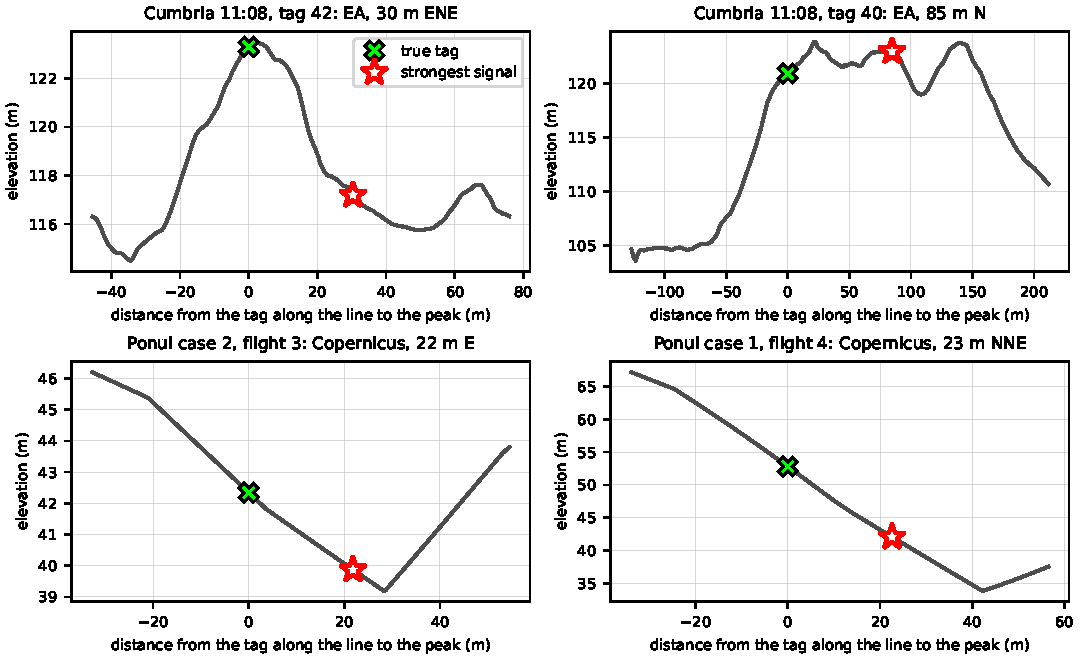
\includegraphics[width=0.95\textwidth]{fieldreview-terrain}
\caption{Terrain along the line from the true tag through the strongest signal, from the
\SI{1}{m} EA model (Cumbria) and the \SI{30}{m} Copernicus model (Ponui).}
\label{fig:terrain}
\end{figure}

On every well-sampled flight where the tag was inside the flown area the peak is lower than
the tag: \SIrange{3}{7}{m} on the three Cumbria tag 42 surveys, \SI{2.5}{m} on the final Ponui
case 2 flight, \SI{11}{m} and \SI{19}{m} on the last two case 1 flights. The one flight where the tag was
outside the survey (tag 40) is the exception, and there the offset is the survey geometry.
This is consistent with the paper's account and its \SIrange{20}{30}{m} residuals. It is also
why the report never calls the position a tag position: a biologist reading ``strongest
signal, \SI{30}{m}, downhill'' will walk uphill from it, which is right.

\subsection{Sensitivity to grid spacing and smoothing}
\label{sec:sensitivity}

\begin{figure}[htbp]
\centering
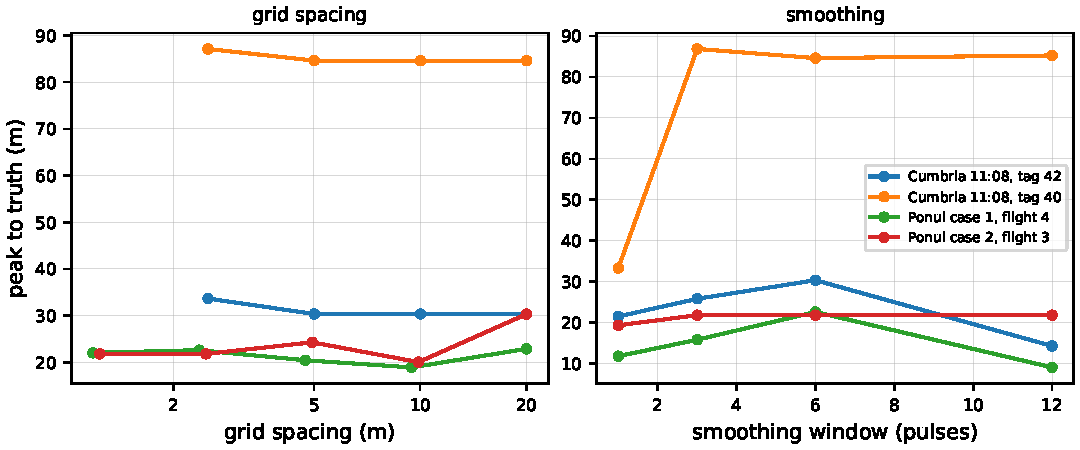
\includegraphics[width=0.95\textwidth]{fieldreview-sensitivity}
\caption{Distance from the strongest signal to the true tag as the grid spacing (left) and
the smoothing window (right) are varied, four cases.}
\label{fig:sensitivity}
\end{figure}

\begin{table}[htbp]
\centering
\resizebox{0.9\textwidth}{!}{\begin{tabular}{lrlrrrr}
\toprule
Case & Grid (m) &  & Peak shift (m) & Bearing shift & Offset (m) & Lobes \\
\midrule
Cumbria 11:08, tag 42 & 2.5 & rule $\times$ 0.5 & 4 & -0 & 34 & 1 \\
Cumbria 11:08, tag 42 & 5.0 & rule $\times$ 1 & 0 & +0 & 30 & 1 \\
Cumbria 11:08, tag 42 & 10.0 & rule $\times$ 2 & 0 & +0 & 30 & 1 \\
Cumbria 11:08, tag 42 & 20.0 & rule $\times$ 4 & 0 & +2 & 30 & 1 \\
Cumbria 11:08, tag 40 & 2.5 & rule $\times$ 0.5 & 3 & +0 & 87 & 2 \\
Cumbria 11:08, tag 40 & 5.0 & rule $\times$ 1 & 0 & +0 & 85 & 2 \\
Cumbria 11:08, tag 40 & 10.0 & rule $\times$ 2 & 0 & +1 & 85 & 2 \\
Cumbria 11:08, tag 40 & 20.0 & rule $\times$ 4 & 0 & +2 & 85 & 2 \\
Ponui case 1, flight 4 & 1.2 & rule $\times$ 0.5 & 2 & +2 & 22 & 2 \\
Ponui case 1, flight 4 & 2.4 & rule $\times$ 1 & 0 & +0 & 23 & 2 \\
Ponui case 1, flight 4 & 4.7 & rule $\times$ 2 & 2 & -5 & 20 & 2 \\
Ponui case 1, flight 4 & 9.5 & rule $\times$ 4 & 5 & -7 & 19 & 1 \\
Ponui case 1, flight 4 & 20.0 & fixed & 10 & +3 & 23 & 1 \\
Ponui case 2, flight 3 & 1.2 & rule $\times$ 0.5 & 0 & -7 & 22 & 1 \\
Ponui case 2, flight 3 & 2.5 & rule $\times$ 1 & 0 & +0 & 22 & 1 \\
Ponui case 2, flight 3 & 4.9 & rule $\times$ 2 & 2 & +2 & 24 & 1 \\
Ponui case 2, flight 3 & 9.9 & rule $\times$ 4 & 6 & +3 & 20 & 2 \\
Ponui case 2, flight 3 & 20.0 & fixed & 22 & -7 & 30 & 2 \\
\bottomrule
\end{tabular}
}
\caption{Grid spacing from half to four times the rule, plus fixed values. Peak shift and
bearing shift are relative to the rule's own result.}
\label{tab:sensitivity}
\end{table}

Grid spacing barely matters, as the vertex argument predicts: over an eightfold range the
peak moves by at most a cell or two, the offset to truth stays within \SI{4}{m} on Cumbria
and \SI{8}{m} on Ponui, and the bearing moves by under \SI{8}{\degree}. Smoothing matters more,
because it is what decides which pulse is the strongest: the offset ranges \SIrange{14}{30}{m}
on tag 42 and \SIrange{33}{87}{m} on tag 40 as the window goes from 1 to 12 pulses. The bench
default of 6 is kept; it belongs in the configuration menu, not on the screen.

\subsection{Contours at small scale}

\begin{figure}[htbp]
\centering
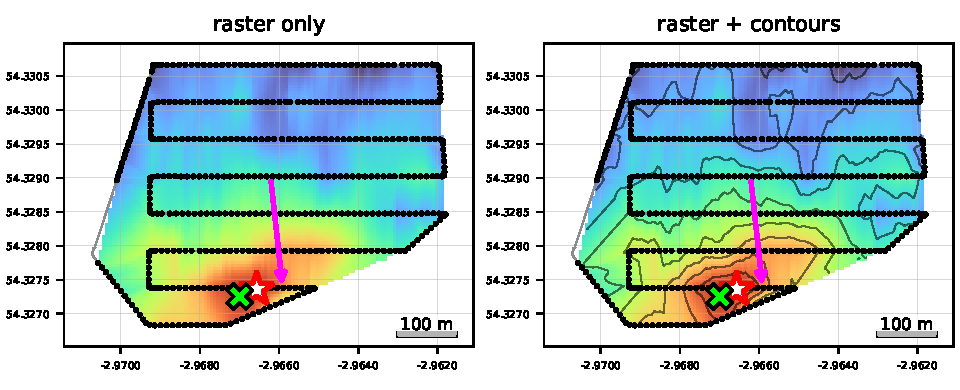
\includegraphics[width=0.9\textwidth]{fieldreview-contours-small}
\caption{The tag 42 surface at roughly the size it would have on a \SI{7}{inch} screen,
without and with contour lines.}
\label{fig:contours}
\end{figure}

At this size the raster carries the message on its own; the contours add the shape of the
peak and the direction of the slope, which is what the bearing is trying to say, and they
do not obscure anything. They are cheap and switchable. Whether they survive sunlight on the
actual Herelink is still a field question, but nothing here argues against carrying them.

\subsection{Two lobes}

\begin{figure}[htbp]
\centering
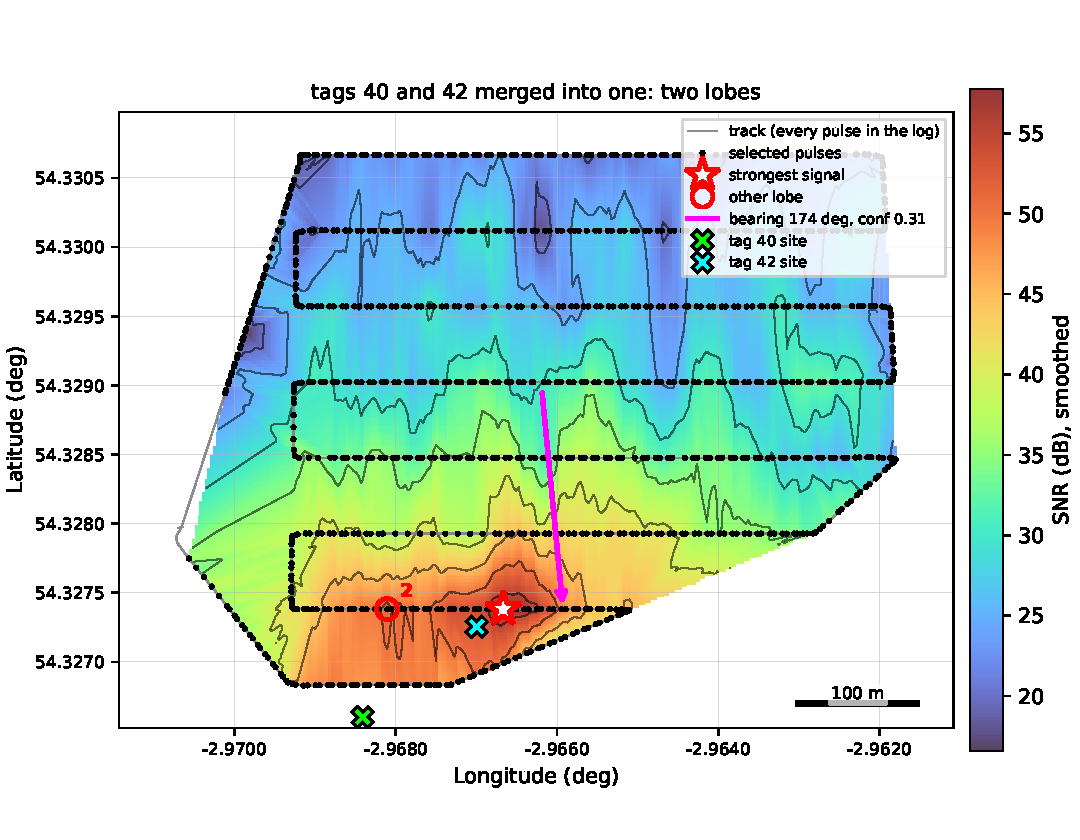
\includegraphics[width=0.85\textwidth]{fieldreview-lobes}
\caption{Cumbria tags 40 and 42, which sit \SI{100}{m} apart, fed to the review as if they
were one tag: what a log with two transmitters on one channel would look like. The report
gives the strongest signal at the tag 42 site and a second lobe \SI{94}{m} west at the tag 40
site, \SI{6.5}{dB} down, out of 163 local maxima on the surface.}
\label{fig:lobes}
\end{figure}

\begin{table}[htbp]
\centering\footnotesize
\begin{tabular}{lrrrrrrrr}
\toprule
Case & Contrast & 3 / 1 & 6 / 1 & 6 / 2 & 10 / 1 & 10 / 2 & 10 / 3 & 15 / 3 \\
\midrule
Cumbria 11:08, tag 42 & 31 dB & 1 & 1 & 1 & 1 & 1 & 1 & 1 \\
Cumbria 11:08, tag 43 (weak) & 5 dB & 1 & 1 & 1 & 1 & 1 & 1 & 1 \\
Cumbria 11:08, tag 40 & 25 dB & 1 & 2 & 2 & 2 & 2 & 2 & 2 \\
Cumbria 11:08, tag 41 (weak) & 9 dB & 8 & 25 & 11 & 25 & 11 & 3 & 7 \\
Cumbria 09:35, tag 42 & 14 dB & 1 & 3 & 2 & 5 & 2 & 2 & 3 \\
Cumbria 09:35, tag 40 (weak) & 8 dB & 1 & 5 & 3 & 6 & 4 & 2 & 3 \\
Cumbria 13:05, tag 42 & 27 dB & 1 & 1 & 1 & 1 & 1 & 1 & 1 \\
Cumbria 13:05, tag 40 & 23 dB & 1 & 2 & 2 & 2 & 2 & 2 & 4 \\
Cumbria 14:12, tag 42 & 21 dB & 1 & 1 & 1 & 1 & 1 & 1 & 2 \\
Cumbria 14:12, tag 40 & 19 dB & 2 & 2 & 1 & 2 & 1 & 1 & 1 \\
Ponui case 1, flight 1 & 21 dB & 1 & 2 & 2 & 2 & 2 & 2 & 3 \\
Ponui case 1, flight 2 (weak) & 9 dB & 2 & 3 & 1 & 6 & 4 & 2 & 2 \\
Ponui case 1, flight 3 & 16 dB & 1 & 1 & 1 & 2 & 2 & 2 & 4 \\
Ponui case 1, flight 4 & 15 dB & 1 & 1 & 1 & 2 & 2 & 1 & 1 \\
Ponui case 2, flight 1 (weak) & 7 dB & 1 & 3 & 2 & 3 & 2 & 1 & 1 \\
Ponui case 2, flight 2 & 17 dB & 1 & 2 & 1 & 2 & 1 & 1 & 1 \\
Ponui case 2, flight 3 & 18 dB & 1 & 1 & 1 & 1 & 1 & 1 & 1 \\
Cumbria 11:08, tags 40+42 merged & 28 dB & 1 & 1 & 1 & 4 & 2 & 1 & 1 \\
\bottomrule
\end{tabular}

\caption{Number of lobes each case reports as the window $W$ / prominence floor $P$ (dB)
vary, uncapped. The defaults are $10/2$.}
\label{tab:lobes}
\end{table}

\section{Answers to the specification's questions}
\label{sec:answers}

\begin{enumerate}
\item \textbf{What grid spacing rule works across a tight rotation and a wide lawnmower?}
Equation~\eqref{eq:spacing}: half the median pulse spacing, held between 60 and 300 cells
across the longer side. It chose \SIrange{2.2}{7.4}{m} on every survey on disk and fell back to
the extent bound only on a \SI{67}{m} lawnmower and on a log with duplicated positions. The
position reported does not depend on it in any case.
\item \textbf{Do contours read at small scale, or is the raster enough?} The raster is
enough to find the peak; the contours add shape and cost nothing. Keep them, switchable.
\item \textbf{What does the peak finder do with two lobes?} Reports both, ranked, with the
second's distance, direction, depth below the first and prominence, using topographic
prominence to tell a lobe from a wrinkle. Thresholds \SI{10}{dB} window, \SI{2}{dB} prominence,
three lobes at most, from Table~\ref{tab:lobes}.
\item \textbf{How far is the reported peak from truth, and is it downhill?}
\SIrange{22}{41}{m} on well-sampled Cumbria flights, \SI{22}{m} on the final Ponui case 2
flight, \SI{23}{m} on the final case 1 flight; lower than the tag in every one of those, by
\SIrange{2.5}{19}{m}.
\end{enumerate}

\section{For the TagTracker delivery}

\begin{itemize}
\item The analysis core is six functions with no GUI dependency and runs in under
\SI{0.2}{s} per flight on a laptop at \SIrange{6}{80}{k} cells; the Herelink will be slower
but the budget is generous.
\item \textbf{Show the real track.} Here the track is the positions of every pulse in the
log, because that is all the CSV holds. Inside TagTracker the vehicle position is free.
\item Keep the caveat, the weak flag and the edge flag on the screen; they were right on
every flight in the validation.
\item The spatial box matters more than it looked. The convex hull stretches the surface over
never-flown wedges wherever there is a transit leg (Figure~\ref{fig:ponui2}); a box is the
one-gesture fix.
\item Show the bearing with its confidence, and expect it to be low on a bullseye.
\end{itemize}

\section{Caveats and open items}

\begin{itemize}
\item The 2023 logs write timestamps to six significant figures, so a whole flight shares one
or two values; the time window and takeoff trim are meaningless on them.
\item The confirmed-only filter cannot be tested on any log on disk.
\item Copernicus is a surface model; on forested Ponui the terrain profiles include canopy.
\item Prominence is implemented in a Python loop; the C++ port is straightforward.
\item MATLAB was never run. All verification is Python against real logs and synthetic
surfaces with known answers; \code{test\_fieldreview.py} and \code{test\_core.py} both pass.
\end{itemize}

\appendix
\section{Command line}

\begin{lstlisting}
python fieldreview.py LOG [--tag ID] [--time START END] [--no-trim] [--alt LO HI]
                          [--box LAT0 LAT1 LON0 LON1] [--all] [--smooth N] [--grid M]
                          [--levels N] [--within-db DB] [--min-prominence DB]
                          [--max-peaks N] [--min-separation M] [--truth LAT LON]
                          [--png FILE] [--json FILE] [--show]
\end{lstlisting}

\code{--time} is minutes from the first pulse of the log. \code{--json} writes everything
in the report plus the peaks, contours in lat/lon and the bearing, for another program to
consume.

\section{Regenerating this document}

\begin{lstlisting}
cd DOCS
make fieldreview-figures      # runs ../python/validate_fieldreview.py; needs the logs
make fieldreview-prototype.pdf
\end{lstlisting}

The terrain checks download two rasters on first use into \code{python/data/dem/}
(gitignored): the EA box for Cumbria and the Copernicus tile for Ponui. Pass
\code{--no-dem} to \code{validate\_fieldreview.py} to skip them.

\end{document}
